\documentclass[conference]{IEEEtran}
\IEEEoverridecommandlockouts

\usepackage{cite}
\usepackage{graphicx}
\usepackage{booktabs}
\usepackage{array}
\usepackage{url}
\usepackage[T1]{fontenc}
\usepackage{textcomp}

% Straight quotes and safe verbatim-in-text for code tokens.
\usepackage{upquote}
\newcommand{\code}[1]{\texttt{#1}}

\begin{document}

\title{Byte-Preserving Response Splitting to Obfuscate the Segmentation
Fingerprint of DNP3 Outstations}

\author{\IEEEauthorblockN{Author Name(s)}
\IEEEauthorblockA{Affiliation \\ Email address}}

\maketitle

\begin{abstract}
A passive observer that watches DNP3 traffic can fingerprint an outstation from
the size, segmentation, and timing of its responses, even without decoding the
payload. Preventing this fingerprinting is challenging, because DNP3 outstations
segment their responses deterministically and any change to the response bytes
breaks the per-block cyclic redundancy checks (CRCs) that the master validates.
In this paper, we propose CRC-boundary splitting, a byte-preserving obfuscation
primitive that re-segments a captured DNP3 response only on its existing CRC
block boundaries. No DNP3 byte is modified and no CRC is recomputed, so the
concatenation of the emitted chunks equals the original response, and the live
master reassembles the identical application message. We implement CRC-boundary
splitting in a request-aware split-replay server that stands in for the
outstation, and we evaluate it on a two-host testbed with an OpenDNP3 master and
outstation. A large Class~0 read that OpenDNP3 natively delivers as 9~application
fragments across 49~link frames and 20~TCP segments can instead be presented as
up to 141~chunks of at most 18~bytes, while the master still delivers all
measurements and returns a DNP3 CONFIRM on a connection with zero
retransmissions and zero resets. Across a granularity sweep, the master accepted
every splitting level and produced measurements identical to the baseline. Based
on these results, we believe that byte-preserving CRC-boundary splitting holds
promise as the transparent primitive for an in-network obfuscation layer that
resists passive fingerprinting of DNP3 outstations.
\end{abstract}

\begin{IEEEkeywords}
DNP3, SCADA, traffic obfuscation, device fingerprinting, industrial control
systems.
\end{IEEEkeywords}

\section{Introduction}

Supervisory control and data acquisition (SCADA) systems that operate power grids
exchange measurement and control data over legacy protocols such as DNP3
(Distributed Network Protocol~3)~\cite{ref:dnp3}. These protocols typically carry
no encryption and no authentication by default~\cite{ref:dnp3}, so any observer on
the communication path can read the traffic. In December~2015, remote intruders
penetrated a Ukrainian power grid and caused a blackout that affected 225{,}000
residents~\cite{ref:ukraine}. Before an adversary can inflict such damage, it
first observes the target to learn what the devices are and how they behave.
Consequently, the information a passive observer can extract from unencrypted
control traffic is a real security concern, and not only in theory.

A passive observer does not need to decode the DNP3 payload to learn about a
device. Traffic-analysis studies have shown that packet sizes and timing alone
can identify the content of even encrypted communications~\cite{ref:fp}, and
unencrypted DNP3 traffic exposes a similar side channel. The size of an
outstation's response, the number of frames it is split into, and the timing
between those frames form a fingerprint of the device and its database. For
example, a large integrity poll produces a long, highly segmented response, while
a small point read produces a short one, so the observed segmentation pattern
already reveals how many points the device exposes. This fingerprint can be
stable across sessions, because a DNP3 outstation segments its responses
deterministically according to the protocol's frame structure. Consequently, an
observer can distinguish device types, infer database sizes, and track a device
across sessions, all without breaking any encryption.

Hiding this fingerprint is challenging, due to two reasons. First, DNP3 protects
every 16-byte block of an application message with a CRC, and the master
validates these CRCs during reassembly, so any modification of the response
bytes, any inserted padding, or any recomputed length field risks a CRC failure
that the master rejects. Second, the outstation firmware is fixed and
vendor-supplied, so a practical defense cannot change how the device itself
builds its frames. There exists a research gap for an obfuscation primitive that
alters the wire-visible size and segmentation of a DNP3 response while preserving
the exact bytes the master expects to reassemble.

In this paper, we propose CRC-boundary splitting, a byte-preserving obfuscation
primitive that changes how a DNP3 response is segmented on the wire without
changing a single DNP3 byte. The idea is to cut the response into TCP chunks only
on the boundaries between the CRC-protected blocks that already exist in the
captured stream. Because every chunk ends on an already-valid CRC and the chunks
concatenate back to the original response, the master reassembles the identical
application message regardless of how finely the response is chopped. We realize
the primitive in a request-aware split-replay server that stands in for the
outstation, replays the captured responses matched to each master request, and
splits every data response on its CRC boundaries.

To validate the primitive on real DNP3 software, we build a software harness
around an OpenDNP3 master and outstation and evaluate it on a two-host testbed.
This paper makes the following contributions.

\begin{itemize}
\item \textbf{Characterizing the native fingerprint.} We measure how an OpenDNP3
outstation natively segments its responses on a real testbed. A large all-types
read produces a 12{,}204-byte response carried as 9~application fragments,
49~link frames, and 20~TCP segments, and the response size grows linearly at
about 5.7~bytes per analog point, so the segmentation pattern directly encodes
the database read.
\item \textbf{Byte-preserving CRC-boundary splitting.} We design an obfuscation
primitive that re-segments a captured response only on existing DNP3 CRC block
boundaries, with no CRC recompute and no field modification, such that the
concatenation of the emitted chunks is byte-identical to the original response.
\item \textbf{A request-aware split-replay server.} We implement a replay server
that reassembles whole DNP3 frames from the TCP stream, matches each request by
function code and application sequence, replies only with the matching captured
response, and preserves the DNP3 CONFIRM handshake, so it can stand in for the
outstation without a live proxy.
\item \textbf{Rig evaluation of transparency and correctness.} We show on the
testbed that the master accepts every splitting granularity, delivers
measurements identical to the baseline at the byte, protocol, and measurement
levels, and keeps the TCP connection clean, while the same response is presented
as up to 141~tiny segments instead of the outstation's native 9~frames.
\end{itemize}

\section{Background and Threat Model}

In this section, we first present the DNP3 response structure that makes the
segmentation fingerprint possible. Then we describe the passive-observer threat
model considered in this work.

\subsection{DNP3 response structure}

DNP3 is a request-response protocol used between a master and an outstation in
SCADA systems~\cite{ref:dnp3}. The master issues a read request, e.g., a Class~0
integrity poll, and the outstation returns the requested measurements. A DNP3
message is layered, and each layer imposes its own size limit. At the application
layer, the outstation builds a response fragment that carries the measurement
objects. At the transport layer, a fragment larger than a single segment is split
into transport segments marked with first (FIR) and final (FIN) bits. At the
data-link layer, each transport segment is carried in one or more link frames. A
DNP3 link frame has a fixed structure~\cite{ref:dnp3}: an 8-byte header, a 2-byte
header CRC, and then up to 250~bytes of user data protected by a CRC after every
16-byte block. Consequently, a full link frame reaches a ceiling of 292~bytes,
and a long application response can only be delivered as a run of 292-byte link
frames followed by a shorter tail frame.

The per-block CRCs are the reason byte-preserving splitting is possible at all.
Because every 16-byte block already ends with a valid 2-byte CRC in the captured
stream, a cut placed on such a block boundary produces two pieces that each end
on an already-valid CRC, without recomputing anything.

\subsection{Threat model}

We consider a passive on-path observer. We assume that the adversary can capture
the unencrypted DNP3 traffic between a master and an outstation, e.g., from a
mirrored switch port or a tap on the control network, but does not modify,
inject, or block any packet. We argue that this is a reasonable assumption, as
DNP3 commonly runs without encryption or authentication over shared substation
and utility networks, so read access to the traffic is practical for an adversary
that has established a foothold on the network. The adversary's objective is
reconnaissance: to fingerprint the outstation and infer its type and
configuration from the observable properties of its responses, i.e., response
size, the number and sizes of frames, and inter-frame timing, without decoding
the application payload.

We do not consider an adversary that decrypts a protected channel, because the
observable size and segmentation properties persist even under some tunneling,
and an unencrypted deployment is the practical baseline for legacy DNP3. We also
do not consider an active adversary that tampers with the traffic in this work,
and we leave a defense against active manipulation to future work.

\section{CRC-Boundary Splitting}

In this section, we describe CRC-boundary splitting and the request-aware
split-replay server that realizes it. Fig.~\ref{fig:arch} presents the design.

\begin{figure*}[t]
\centering
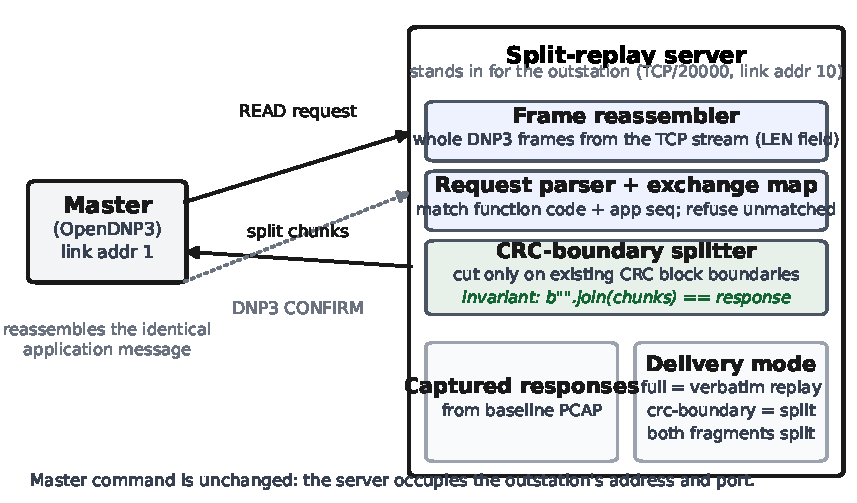
\includegraphics[width=0.86\textwidth]{figures/fig1_architecture.pdf}
\caption{The request-aware split-replay server stands in for the outstation. It
reassembles whole DNP3 frames from the TCP stream, matches each request to its
captured response, splits data responses only on existing CRC block boundaries,
and preserves the CONFIRM handshake. The master command is unchanged.}
\label{fig:arch}
\end{figure*}

\noindent\textbf{The primitive.} CRC-boundary splitting cuts a captured DNP3
response into TCP chunks only on the boundaries between its CRC-protected blocks.
To split a response, we scan it into its sequence of blocks, i.e., the 10-byte
link header block and the following 16-byte data blocks, each already terminated
by its CRC, and we group a configurable number of whole blocks into each TCP
chunk. Because a chunk always begins and ends on a block boundary, every chunk
ends on an already-valid CRC, and the chunks concatenate back to the original
response. Before sending, the server enforces the byte-preservation invariant
\code{b"".join(chunks) == response}; it refuses to send if the check fails.
Consequently, no DNP3 byte is modified, no CRC is recomputed, and no length field
is touched, so the master's link-layer and transport-layer reassembly proceeds
exactly as it does for the native response.

\noindent\textbf{Splitting granularity.} The number of whole blocks per chunk is
the single control knob for how aggressively the response is fragmented. When the
count is one, every CRC block becomes its own TCP segment, which is the most
aggressive byte-preserving split possible; larger counts group more blocks per
write and produce a coarser split. Cutting finer than one block per chunk is not
possible without splitting inside a CRC block, which would break a boundary and
fall outside the byte-preserving primitive. The server also delays each chunk by
a configurable interval, so the timing dimension of the fingerprint can be varied
independently of the size dimension.

\noindent\textbf{Request-aware replay.} The split-replay server stands in for the
outstation at the same address and port, so the master command does not change.
To reply correctly without running a full DNP3 stack, the server reassembles
whole DNP3 frames from the TCP stream using the link-header length field, parses
each request's function code and application sequence, and replies with only the
captured response that matches that request. Because a captured session contains
startup and handshake exchanges as well as the data read, matching each request
to its own captured response keeps the master on its captured trajectory. The
server refuses to fire a captured response at a request it cannot match, which
prevents the blind byte-dumping behavior that an earlier positional replay design
exhibited. Only the data responses are split on CRC boundaries; the short
handshake replies are sent whole.

\noindent\textbf{Handling multi-fragment responses and CONFIRM.} A large read is
answered by more than one application fragment. The outstation sends the first
fragment, the master returns a DNP3 CONFIRM, and the outstation then sends the
continuation fragment. The server preserves this handshake: it sends the split
first fragment, waits for the master's CONFIRM bytes, and then sends the
continuation fragment, split on its own CRC boundaries. Consequently, the
continuation is obfuscated to the same degree as the first fragment rather than
being emitted as a single write.

\section{Implementation}

We implement the harness in Python around an OpenDNP3~\cite{ref:opendnp3}
outstation and master, reached through the ChargePoint pydnp3 binding. The
outstation runner (\code{run\_outstation.py}) starts a real OpenDNP3 outstation
with a configurable database, disables unsolicited responses, and rejects
controls by default, so the baseline capture contains only the issued reads. The
master runner (\code{run\_master.py}) issues one controlled Class~0 read and
writes the delivered measurements to a per-phase CSV together with a
human-readable measurement receipt. All lab settings, i.e., host addresses, TCP
port, and DNP3 link addresses, are read from a single configuration module, so no
address is typed on the command line.

The split-replay server (\code{split\_server.py}) needs no DNP3 stack. It
contains a frame reassembler, a request parser, the CRC-boundary splitter, and a
captured-exchange map, and it depends only on itself and the configuration
module. It exposes two delivery modes: \code{full} replays each captured response
verbatim, and \code{crc-boundary} splits every data response on its CRC
boundaries. The byte-preservation check runs on every response before it is sent.
The harness is deliberately confined to the byte-preserving phase: it recomputes
no CRC, modifies no DNP3 field, inserts no padding, and runs no live proxy, so
that byte preservation stays the enforced invariant throughout.

\section{Evaluation}

In this section, we evaluate CRC-boundary splitting on the testbed. Our
evaluation answers three questions. First, how does an OpenDNP3 outstation
natively segment its responses, i.e., what is the fingerprint we aim to
obfuscate? Second, does the master still accept and correctly reassemble a
response that has been split on CRC boundaries? Third, how far can the size and
segmentation of a response be distorted while preserving byte-level acceptance?

\noindent\textbf{Testbed.} The testbed is two directly switched hosts on a
1~Gb/s management network. The master runs on one host and the outstation, or the
split-replay server in its place, runs on the other on TCP port~20000. The DNP3
link addresses are 1 for the master and 10 for the outstation. We capture the
traffic on the master's interface with a port filter and analyze the captures
with scapy and a DNP3 CRC helper. The outstation and master use OpenDNP3 through
pydnp3 on Python~3.12. Unless stated otherwise, all results are from the two-host
rig, not from loopback.

\subsection{Native segmentation fingerprint}

To characterize the fingerprint, we issue a single large Class~0 read against an
outstation configured with 200~analog, 50~binary, and 50~counter points, and we
measure the response from the capture. Table~\ref{tab:baseline} presents the
result. The outstation returns a 12{,}204-byte response carried as
9~application fragments, 49~link frames, and 20~TCP segments. Of the 49~link
frames, 46 are the 292-byte DNP3 maximum and the remainder are short per-fragment
tails. The reason the response reaches 49~link frames is that 292~bytes is the
DNP3 link-frame ceiling, so a long application fragment can only be delivered as
a run of full frames plus a short tail.

\begin{table}[t]
\centering
\caption{Native segmentation of a large Class~0 read (200 analog + 50 binary +
50 counter).}
\label{tab:baseline}
\begin{tabular}{@{}p{0.62\columnwidth}r@{}}
\toprule
Layer & Result \\
\midrule
Total response bytes (outstation to master) & 12{,}204 \\
DNP3 application fragments (transport FIR/FIN) & 9 \\
DNP3 link frames (\code{0x0564}) & 49 \\
Link frame sizes & $46 \times 292$\,B + tails \\
TCP segments (response) & 20 \\
\bottomrule
\end{tabular}
\end{table}

The DNP3 layer and the TCP layer segment independently. The kernel packs the link
frames into TCP segments of up to 1448~bytes, i.e., the connection's maximum
segment size, so a single 292-byte link frame can straddle a TCP segment boundary
and a single TCP segment can carry several partial link frames. Consequently, the
two segmentation boundaries do not align, and the wire-visible pattern reflects
both the DNP3 frame structure and the TCP packing.

To confirm that the fingerprint tracks the database, we sweep the read range on a
200-analog database and measure the response for each range.
Table~\ref{tab:range} presents the result. The response size grows linearly at
about 5.7~bytes per analog point, and the frame and segment counts rise once the
response crosses the 292-byte frame ceiling and the maximum segment size.
Consequently, a passive observer can infer how many points a device exposes
directly from the size and segmentation of its response, which is the fingerprint
that CRC-boundary splitting aims to obfuscate. An observer may also combine this
size estimate with the response timing to strengthen the fingerprint.

\begin{table}[t]
\centering
\caption{Response size versus read range on a 200-analog database.}
\label{tab:range}
\begin{tabular}{@{}lrrrr@{}}
\toprule
Read range & Analog pts & Bytes & Link frames & TCP segs \\
\midrule
0..9   & 10  & 129   & 4 & 4 \\
0..49  & 50  & 332   & 3 & 3 \\
0..99  & 100 & 625   & 4 & 3 \\
0..199 & 200 & 1{,}211 & 6 & 3 \\
\bottomrule
\end{tabular}
\end{table}

We also measure the outstation's TCP-level response behavior on the same large
read. The outstation piggybacks the application response on the TCP
acknowledgment for 9 of 9~requests, with a mean request-to-acknowledgment delay
of 0.24~ms and a mean request-to-response delay of 1.01~ms, and the steady-state
data segments carry a \code{NOP-NOP-Timestamp} TCP option signature. This is the
host's TCP/IP stack fingerprint, which is distinct from the DNP3 application
fingerprint and would differ for a field device with a different stack.

\subsection{Transparency and correctness of CRC-boundary splitting}

To test whether the master accepts a split response, we run the full pipeline on
the rig. We first capture a baseline read against the real outstation, we extract
the captured responses, and we then replace the outstation with the split-replay
server and repeat the read, once with verbatim replay and once with CRC-boundary
splitting. We compare the delivered measurements across the three runs.

The master accepts the split response and reassembles the identical application
message. When a captured 2{,}407-byte read response, which OpenDNP3 natively
carries as 9~link frames, is delivered as 141~chunks of at most 18~bytes under
one-block-per-chunk splitting, the master still delivers all 800~measurements
from the replayed response set and returns a DNP3 CONFIRM. The measurement sets
are identical at three levels. First, the split bytes concatenate to the original
response, i.e., byte level. Second, the master raises no DNP3 parser or CRC error
and sends the CONFIRM, i.e., protocol level. Last, the delivered measurements
match the baseline, i.e., measurement level. We also ran a clean-pipeline check
on a Class~0 read that returned 2{,}400 unique measurement tuples across a
6-fragment response. The baseline, the verbatim replay, and the CRC-boundary
split produced byte-identical measurement sets, and every data fragment was split
while the handshake replies were left whole. The reason the measurements are
preserved is that CRC-boundary splitting changes only where the TCP write
boundaries fall, which the master's reassembly is indifferent to, and leaves
every DNP3 byte and CRC untouched.

\subsection{Obfuscation envelope}

To measure how far the fingerprint can be distorted, we replay the same captured
2{,}407-byte response split at one, two, four, and eight blocks per chunk,
holding everything else constant. Table~\ref{tab:sweep} presents the result, and
Fig.~\ref{fig:split} shows the size and segmentation distortion against the
native response.

\begin{figure*}[t]
\centering
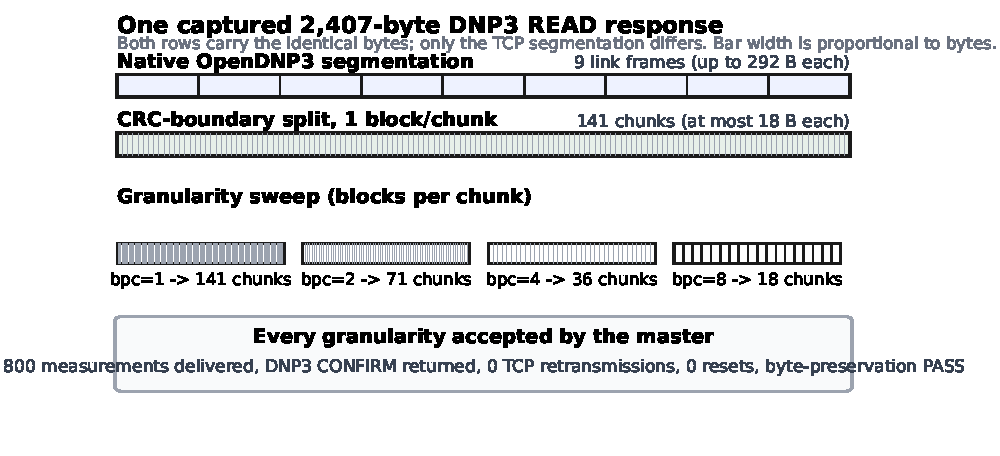
\includegraphics[width=0.86\textwidth]{figures/fig2_baseline_vs_split.pdf}
\caption{The same 2{,}407-byte response carries the identical bytes in both rows;
only the TCP segmentation differs. OpenDNP3 natively presents it as 9~link
frames, while one-block-per-chunk CRC-boundary splitting presents it as
141~chunks of at most 18~bytes. Across the granularity sweep the master accepted
every level, delivering all 800~measurements with a CONFIRM on a clean
connection.}
\label{fig:split}
\end{figure*}

\begin{table}[t]
\centering
\caption{Split-aggressiveness sweep on a captured 2{,}407-byte READ response
(9 native link frames).}
\label{tab:sweep}
\begin{tabular}{@{}rrrrrr@{}}
\toprule
Blocks/chunk & Chunks & Meas. & CONFIRM & Retx & Resets \\
\midrule
1 & 141 & 800 & yes & 0 & 0 \\
2 & 71  & 800 & yes & 0 & 0 \\
4 & 36  & 800 & yes & 0 & 0 \\
8 & 18  & 800 & yes & 0 & 0 \\
\bottomrule
\end{tabular}
\end{table}

The master accepts every granularity and delivers all 800~measurements. It
returns a CONFIRM on a connection with zero retransmissions and zero resets, while
the READ response is presented as 141, 71, 36, and 18~chunks respectively. The
chunk counts follow the ceiling of 141 divided by the blocks-per-chunk value
exactly. Consequently, the byte-preserving obfuscation envelope spans the full
block-grouping range, and the maximum size and segmentation distortion is reached
at one block per chunk, where a single 2{,}407-byte response that the outstation
natively presents as 9~frames is instead presented as 141~tiny segments. Pushing
fragmentation past this point, or changing per-frame sizes arbitrarily, would
require rebuilding frames and recomputing CRCs, which falls outside the
byte-preserving primitive.

\section{Discussion}

\noindent\textbf{From harness to in-network defense.} The harness proves the
primitive in software, where the split-replay server stands in for the outstation
and replays captured responses. It is not yet the final in-network
implementation. A deployed defense would apply CRC-boundary splitting to live
responses in the data plane, e.g., on a programmable switch, rather than
replaying captured ones. We leave the in-network, live implementation and its
throughput and latency evaluation to future work.

\noindent\textbf{What the primitive does and does not hide.} CRC-boundary
splitting distorts the size and segmentation of a response and, through the chunk
delay, its timing, while preserving the DNP3 bytes. It does not change the total
number of bytes the application response carries, so an observer that counts
total payload bytes across a full exchange can still estimate the read size.
Making the total size itself less informative requires padding or frame
rebuilding, which recomputes CRCs and is a separate line from the byte-preserving
primitive studied here. We leave a padding-based extension, and its interaction
with the master's reassembly, to future work.

\noindent\textbf{Scope of the evaluation.} Our fingerprinting measurements
characterize a single outstation on one testbed, so they show what the primitive
changes on the wire rather than a measured reduction in an adversary's
classification accuracy across devices. A quantitative fingerprinting study
across multiple device types and stacks would let us report the obfuscation
effect as a drop in classification accuracy. We leave such a study to future
work.

\section{Related Work}

\noindent\textbf{Traffic obfuscation for ICS reconnaissance.} Prior work
obfuscates control-network communication to disrupt an adversary's reconnaissance
of power grids. In~\cite{ref:raincoat}, the authors randomize data acquisitions
and craft decoy measurements to mislead attackers into designing ineffective
strategies, and in~\cite{ref:defrec}, the authors virtualize physical devices to
disrupt reconnaissance of the cyber-physical infrastructure. These approaches
obfuscate the content and connectivity that an adversary learns. This work, on
the other hand, serves a different objective: it obfuscates the wire-visible size
and segmentation of a DNP3 response without changing any application byte, so it
complements content-level obfuscation rather than replacing it.

\noindent\textbf{Website and traffic fingerprinting defenses.} A large body of
work fingerprints encrypted traffic from packet sizes and timing, and defends
against it by padding and by reshaping the packet-size
distribution~\cite{ref:fp}. The size and segmentation of DNP3 responses give a
similar side channel in an unencrypted industrial setting. Compared to general
traffic-shaping defenses, CRC-boundary splitting is constrained by the DNP3 CRC
structure: it can re-segment freely on block boundaries but cannot alter bytes or
sizes without recomputing CRCs, so it trades some reshaping freedom for exact
byte preservation and transparent master acceptance.

\noindent\textbf{DNP3 security and monitoring.} Prior work adds intrusion
detection and specification-based monitoring to DNP3 traffic~\cite{ref:bro}, and
analyzes the safety impact of malicious DNP3 commands~\cite{ref:cps}. These
efforts detect or analyze malicious activity in the traffic. This work is not a
detection technique: it modifies the outstation's observable traffic to resist
passive fingerprinting, before any malicious activity is attempted.

\section{Conclusion}

A passive observer can fingerprint a DNP3 outstation from the size, segmentation,
and timing of its responses, which are stable because the outstation segments
deterministically and any byte change breaks the protocol's CRCs. In this paper,
we proposed CRC-boundary splitting, a byte-preserving obfuscation primitive that
re-segments a captured response only on its existing CRC block boundaries, and we
implemented it in a request-aware split-replay server. On a two-host testbed, the
master accepted every splitting granularity and delivered measurements identical
to the baseline, while a response that OpenDNP3 natively presents as 9~frames was
presented as up to 141~tiny segments on a connection with zero retransmissions
and zero resets. Based on these results, we believe that CRC-boundary splitting
holds promise as the transparent primitive for an in-network obfuscation layer,
which we plan to implement in the data plane in future work.

% -------------------------------------------------------------------------
% NOTE: the references below are PLACEHOLDERS. Replace each with a complete,
% verified citation before submission. The text names the intended source.
% -------------------------------------------------------------------------
\begin{thebibliography}{1}

\bibitem{ref:dnp3}
IEEE Standard for Electric Power Systems Communications --- Distributed Network
Protocol (DNP3), IEEE Std 1815. [complete citation]

\bibitem{ref:ukraine}
Analysis of the December 2015 Ukraine power grid cyberattack (e.g., E-ISAC/SANS
report). [complete citation]

\bibitem{ref:raincoat}
H.~Lin, Z.~Kalbarczyk, and R.~K. Iyer, ``RAINCOAT: Randomization of network
communication in power grid cyber infrastructure to mislead attackers,'' IEEE
Trans. Smart Grid. [complete citation]

\bibitem{ref:defrec}
H.~Lin \emph{et al.}, ``DefRec: Establishing physical function virtualization to
disrupt reconnaissance of power grids' cyber-physical infrastructures,'' NDSS.
[complete citation]

\bibitem{ref:fp}
Representative website/traffic fingerprinting attack and padding-based defense.
[complete citation]

\bibitem{ref:bro}
H.~Lin \emph{et al.}, ``Adapting Bro into SCADA: Building a specification-based
intrusion detection system for the DNP3 protocol.'' [complete citation]

\bibitem{ref:cps}
H.~Lin \emph{et al.}, ``Safety-critical cyber-physical attacks: Analysis,
detection, and mitigation.'' [complete citation]

\bibitem{ref:opendnp3}
OpenDNP3, an open-source implementation of the DNP3 protocol stack. [complete
citation]

\end{thebibliography}

\end{document}
